\chapter{Theoretical and Computational Methods}


%%%%%%%%%%%%%%%%%%%%%%%%%%%% GENERAL G-EQUATIONS %%%%%%%%%%%%%%%%%%%%%%%%%%%%%%%%%%%%%%%%%%%%
\section{G-Equation Formulation}
\subsection{General G-Equation}
The G-Equation formalism is no more than a mathematical construct of the flame front as an ``infinitesimal'' surface, thus only yields physical representation for flames the have ``thin'' flame fronts. The flame as a mathematical surface, corresponds to a function $G(\vec{x},t)$, that for all points of the flame front $\vec{x}\equiv\vec{x}_f$ in a given time $t$, is equal to constant $G_0$, i.e. the flame front is the level set function has defined in \eqref{lsf}. 
\begin{definition}[\bf{Level Set Function}]
\begin{align}
G(\vec{x}\equiv\vec{x}_f,t)=G_0 &\qquad \text{\bf{unsteady flame front}} \label{lsf}\\
G(\vec{x},t)>G_0 &\qquad \text{\bf{product side}}\nonumber \\
G(\vec{x},t)<G_0 &\qquad \text{\bf{reacting side}}\nonumber \\[3mm]
\text{with} \qquad   G:\mathbb{R}^4 \longrightarrow \mathbb{R},& \quad G_0 \in \mathbb{R}, \quad \vec{x}\in \mathbb{R}^3, \quad t \in \mathbb{R} \nonumber
\end{align}
\comment{should  impose differentiability on g}
\end{definition}	
The knowledge of the level set function is actually of limited practical utility, since nothing relevant is said about the flame front points $\vec{x}_f$ which is the information we desire to obtain. 

\begin{definition}[\bf{Kinematic Relations}]
It is known that the gradient of a differentiable level set function is orthogonal to that level set, therefore the normal vector $\vec{n}$ can be directly calculated from the gradient of $G$ and normalized. The direction points outward, i.e. from the unburnt toward the burnt since it is also the direction of growing $G_0$, see figure \ref{gfig}.
\begin{align}
	\vec{n} \equiv \dfrac{\vec{\nabla G}}{\modu{\vec{\nabla} G}} \label{normal_eq}
\end{align}
Noting that flame front velocity $\vec{u}_f$, is the vectorial sum of the fluid/flow velocity  at the flame front $\left.\vec{u}\right|_{G=G_0}$ and of the laminar burning velocity $-S_L \vec{n}$. This last term being the planar velocity at which the combustion wave would propagate from the burnt gases toward the unburnt mixture (thus the negative sign relative to the normal vector), even if the fluid where at rest, see figure \ref{gfig}. 
\begin{align}
	\vec{u}_f \equiv \left.\vec{u}\right|_{G=G_0} -S_L \vec{n} \label{kine_eq}
\end{align}
\end{definition}

\begin{figure}[h!]
\begin{center}
\includegraphics[scale=1.3]{./img/g_equation}
\end{center}
\caption{Diagram of a cross cut of a premixed burner/injector, acoustically excited, with a single, anchored unsteady flame front (red). The steady flame front (dashed red) is also represented as well a zoom on the flame region, for the analysis of the kinematic relations.}
\label{gfig}
\end{figure}

\begin{theorem}[\bf{General G-Equation}]
Taking the total time derivative of equation \eqref{lsf}, and noting that $G_0$ is a real constant. 
\begin{align}
	\dfrac{d G(\vec{x}_f,t)}{dt}=\dfrac{\partial G}{\partial t} + \dfrac{d \vec{x}_f}{dt} \dfrac{\partial G}{\partial \vec{x}_f}=0 \nonumber \\
	\dfrac{\partial G}{\partial t} + \vec{u}_f \cdot \vec{\nabla} G =0 \label{g_sfeq}
\end{align}
Substituting the flame velocity, \eqref{kine_eq} and flame normal \eqref{normal_eq} into \eqref{g_sfeq}.
\begin{align*}
	\dfrac{\partial G}{\partial t} + \left.\vec{u}\right|_{G=G_0} \cdot \vec{\nabla} G - S_L  \dfrac{\vec{\nabla G} \cdot \vec{\nabla} G}{\modu{\vec{\nabla} G}} =0\\ 
	\dfrac{\partial G}{\partial t} +  \left.\vec{u}\right|_{G=G_0} \cdot \vec{\nabla} G - S_L  \dfrac{\modu{\vec{\nabla} G}^2}{\modu{\vec{\nabla} G}} =0
\end{align*}\vspace{-3mm}
\begin{empheq}[box={\mybluebox[2mm][2mm]}]{align}
\dfrac{\partial G}{\partial t} + \left.\vec{u}\right|_{G=G_0} \cdot \vec{\nabla} G - S_L  \modu{\vec{\nabla} G}=0\label{G_eq}
\end{empheq}
\end{theorem}
\comment{missing boundary conditions (isn't this a cauchy problem???)}

The determination of the points of the flame front are determined from G-equation \eqref{G_eq} and with the help of definition \eqref{lsf}, however the velocity field at the flame front must be prescribed ($ \left.\vec{u}\right|_{G=G_0} $), along side with a value or model for the laminar burning velocity $S_L$.





%%%%%%%%%%%%%%%%%%%%%%%%%%%% SIMPLIFIED G-EQUATIONS %%%%%%%%%%%%%%%%%%%%%%%%%%%%%%%%%%%%%%%%%%%%
\clearpage
\subsection{Simplified G-Equations} 
As mentioned on the previous section, in order to solve the G-equation, either numerically or analytically, a model for the underlying velocity field and model for the laminar burning velocity must be supplied. However there are some simplifying assumptions that can be made to the general G-equation before choosing those models. The chain of assumptions that we are about to make is sequential in most cases, thus generating G-equations of gradually more limiting domains, as seen in figure \ref{equation_flowchart}. Some assumptions have been found to be true experimentally in wide domain of flow circumstances (like axisymmetry), while other have a quite more limited range of applicability (like non-folded or tall flames).

\begin{assumption}[\bf{Axisymmetry}]
Given that a great part of burner and injectors are circular it is usual to represent all the G-equation's functions ($G$,$\vec{u}$ and $S_L$) in cylindrical coordinates. Furthermore since the flows are ''quite regular'' it is assumed that those functions are independent from the angular coordinate $\theta$, and in the case of the flow velocity $u_{\theta}=0$, i.e. axisymmetric.
\begin{align}
	G(\vec{x},t) = G(r,\theta,z,t) &\implies G(r,z,t) \\
	\vec{u}(\vec{x},t)=\vec{u}(r,\theta,z,t)=\begin{bmatrix}  u_r(r,\theta,z,t) \\ u_{\theta}(r,\theta,z,t) \\ u_z(r,\theta,z,t) \end{bmatrix} &\implies \vec{u}(r,z,t)=\begin{bmatrix}  u_r(r,z,t) \\ u_z(r,z,t) \end{bmatrix} \\
	S_L(\vec{x},t)=S_L(r,\theta,z,t) &\implies S_L(r,z,t)
\end{align}
\label{axisym_ass}
\end{assumption}

\begin{theorem}[\bf Axisymmetric G-equation]
Introducing assumption \ref{axisym_ass} into the general G-equation \eqref{G_eq}.
\begin{align*}
	\dfrac{\partial G}{\partial t} + \left. \begin{bmatrix} u_r & u_z \end{bmatrix} \right|_{G=G_0} \cdot \begin{bmatrix} \\[-4mm] \dfrac{\partial G}{\partial r} \\[3mm] \dfrac{\partial G}{\partial z} \end{bmatrix} - S_L  \modu{  \begin{bmatrix} \\[-4mm] \dfrac{\partial G}{\partial r} \\[3mm] \dfrac{\partial G}{\partial z} \end{bmatrix} }=0
	\end{align*}
\begin{empheq}[box={\mybluebox[2mm][2mm]}]{align}
	\dfrac{\partial G}{\partial t} + \left. u_r \right|_{G=G_0}  \dfrac{\partial G}{\partial r} +  \left.  u_z \right|_{G=G_0} \dfrac{\partial G}{\partial z} - S_L \sqrt{ \left(\dfrac{\partial G}{\partial r}\right)^2 + \left(\dfrac{\partial G}{\partial z}\right)^2 }=0 \label{gaxi_eq}
\end{empheq}
\end{theorem}


\begin{assumption}[\bf{Non-Folded Flames}]
If we continue from assumption \ref{axisym_ass}, and assume that the G-function is separable in the $z$ direction.
The g-function is now only function of the radial direction $r$, and time $t$. 
\begin{align}
	G(r,z,t)=z - g(r,t)
	\label{nofold_eq}
\end{align}
This means that the original implicit G-function is now transformed in explicit g-function $g$, which is explicit in the $z$ direction, this can be easily shown by \eqref{lsf}, and \eqref{nofold_eq}.
\begin{align}
	z=&g(r,t)+G_0 \quad \text{on the flame front} \nonumber \\
	z=&g(r,t) \quad \text{on the flame front with} \quad G_0=0 \label{g0_eq}
\end{align}
An relevant observation, that gives name to this assumptions, is if the g-function is to be a function, (the arguments of $g$ have one and only one value), it cannot be folded in the $z$ direction. This assumptions has a limited range of applicability since for strongly deformed flames it has been observed in experimental setups. 
\label{nofold_ass}
\end{assumption}

\begin{theorem}[\bf{Non Folded g-equation}]
Introducing equation \eqref{nofold_eq}, from assumption \ref{nofold_ass}, into equation \eqref{gaxi_eq}, and carrying out the calculations.
\begin{align*}
	\dfrac{\partial z-g}{\partial t} + \left. u_r \right|_{G=G_0}  \dfrac{\partial z-g}{\partial r} +  \left.  u_z \right|_{G=G_0} \dfrac{\partial z-g}{\partial z} - S_L \sqrt{ \left(\dfrac{\partial z-g}{\partial r}\right)^2 + \left(\dfrac{\partial z-g}{\partial z}\right)^2 }=0
\end{align*}

\begin{empheq}[box={\mybluebox[2mm][2mm]}]{align}
	-\dfrac{\partial g}{\partial t} - \left. u_r \right|_{G=G_0}  \dfrac{\partial g}{\partial r} +  \left.  u_z \right|_{G=G_0} - S_L \sqrt{ \left(\dfrac{\partial g}{\partial r}\right)^2 +1 }=0 \label{gnofold_eq}
\end{empheq}
\end{theorem}


\begin{assumption}[\bf{Tall, Monotonic Flames}]
This assumption arises from the need to simplify the modulus and the square root it originates, in the g-equation \eqref{gnofold_eq}. 
\begin{align}
	\left(\dfrac{\partial g}{\partial r}\right)^2&\gg 1  \quad \text{and} \quad \dfrac{\partial g}{\partial r} \leq 0
\end{align}
\label{tall_ass}
\end{assumption}

\begin{theorem}[\bf Tall g-equation]
Imposing the tall flame assumption (\ref{tall_ass}) into the non-folded g-equation \eqref{gnofold_eq}.
\begin{empheq}[box={\mybluebox[2mm][2mm]}]{align}
	-\dfrac{\partial g}{\partial t} - \left. u_r \right|_{G=G_0}  \dfrac{\partial g}{\partial r} +  \left.  u_z \right|_{G=G_0} - S_L \modu{ \dfrac{\partial g}{\partial r}}=0 \label{gtall_eq}
\end{empheq}
\end{theorem}

\begin{assumption}[\bf{Separable, Time Harmonic g-function}]
This assumption arises as way to transform the partial differential g-equation into a ordinary differential equation.
\begin{align}
	g(r,t)=\bar{g}(r) + g'(r)e^{-i\omega t}
\end{align}
\label{sep_g_ass}
\end{assumption}


\begin{theorem}[\bf Non-Folded Ordinary g-equation]
Introducing assumption \ref{sep_g_ass}, into equation \eqref{gnofold_eq}.
\begin{empheq}[box={\mybluebox[2mm][2mm]}]{align}
	i \omega g' e^{-i\omega t} - \left. u_r \right|_{G=G_0}\left( \dfrac{\partial \bar{g}}{\partial r} + \dfrac{\partial g'}{\partial r} e^{-i \omega t} \right) +  \left.  u_z \right|_{G=G_0} - S_L \sqrt{ \left(  \dfrac{\partial \bar{g}}{\partial r} + \dfrac{\partial g'}{\partial r} e^{-i \omega t} \right)^2 +1 }=0 \label{gord_eq}
\end{empheq}
This equation is still strongly coupled between steady and oscillating terms, especially due the terms inside the square root.
\end{theorem}

\begin{theorem}[\bf Tall Ordinary g-equation]
\begin{empheq}[box={\mybluebox[2mm][2mm]}]{align}
	i \omega g' e^{-i\omega t} - \left. u_r \right|_{G=G_0}\left( \dfrac{\partial \bar{g}}{\partial r} + \dfrac{\partial g'}{\partial r} e^{-i \omega t} \right) +  \left.  u_z \right|_{G=G_0} - S_L \modu{ \dfrac{\partial \bar{g}}{\partial r} + \dfrac{\partial g'}{\partial r} e^{-i \omega t} }=0 \label{gtallord_eq}
\end{empheq}
\end{theorem}


\begin{figure}[!h]
\begin{center}
\includegraphics[scale=1.2]{./img/equation_flowchart}
\end{center}
\caption{Flow chart that represents the cascading of simplified G-equations from the most general on top to least on the bottom. It can be used to choose a desired level of approximation, then after reaching the desired level we must always follow up to a modeling of flow velocity and laminar burning velocity.}
\label{equation_flowchart}
\end{figure}
\vspace{8mm}
As summary of this section, we represent all the equations deduced, according to the consecutive assumptions in flowchart \ref{equation_flowchart}. We start with the general G-equation \eqref{G_eq}, the axisymmetric assumptions \ref{axisym_ass} then generates the axisymmetric G-equation \eqref{gaxi_eq}, then we add the non-folded assumption \ref{nofold_ass} and this produces the non-folded g-equation \eqref{gnofold_eq}. From the non-folded g-equation we apply the tall flame assumption \ref{tall_ass} producing the tall g-equation \eqref{gtall_eq}. Finally we apply the g-function separable time harmonic assumption \ref{sep_g_ass}, however this assumption can be applied to both the non-folded g-equation \eqref{gnofold_eq}, and the tall g-equation \eqref{gtall_eq}, producing respectively the non-folded ordinary \eqref{gord_eq}, and tall ordinary \eqref{gtallord_eq}.





%%%%%%%%%%%%%%%%%%%%%%%%%%%% MODELING VELOCITY FIELD %%%%%%%%%%%%%%%%%%%%%%%%%%%%%%%%%%%%%%%%%%%%
\clearpage
\subsection{Modeling Flow Velocity Field}
We can either supply a analytical velocity field or use experimental or computational approaches to obtain the velocity field.
We choose the second approach and provide a analytical flow field that has quite general mathematical form, and also quite ``strong'' experimental evidence.

\begin{assumption}[\bf{Uniaxial, Separable, Traveling Wave Flow Velocity}] 
There have been experimental evidence that radial velocity component is negligible, since by velocimetry techniques (LDV or PIV for example) the flow speed can be determined with quite high precision.
\begin{align}
	u_r=0
\end{align}

For the axial velocity component $u_z$ is possible to express the underlying flow assuming it as a uniform base flow $\bar{u}_z$, and adding a traveling wave in the $z$ direction, with wave number $k$ and angular frequency $\omega$, these kind of general wave like behavior is see in several other physical problems like acoustics, electromagnetism and quantum mechanics.
\begin{align*}
	u_z(r,z,t)=\bar{u}_z(r) + u'_z(r)e^{i(kz - \omega t)}
\end{align*}
The wave number $k$, can be related with a propagation wave phase velocity $v_p$, as well as the relation between angular frequency $\omega$ and wave frequency $f$. 
\begin{align}
	\omega=&2 \pi f\\
	k =&\dfrac{\omega}{v_p}= \dfrac{2\pi f}{v_p}
\end{align}
Thus axial velocity is given by:
\begin{align}
	u_z(r,z,t)=\bar{u}_z(r) + u'_z(r)e^{i\omega\left(\dfrac{z}{v_p}\ -\ t\right)}
\end{align}
\label{u_ass}
\end{assumption}

The angular frequency $\omega$ is usually a input for the system, as we will see further on the flame transfer functions, from experimental point of view it is this frequency that is set on the loudspeaker the excites the system, in order to generate the velocity oscillation. 
However the wave phase velocity $v_p$ is a little more debatable since from a physical point of view, what would make sense is that should be about the same has the flow average velocity $\bar{u}_z$, however from a acoustic point of view it is interesting to note that a wave is also generated on top of this flow, and it propagates with the speed of sound $c$, however with a much smaller amplitude.

\comment{some suggest that $v_p\not= \bar{u}_z$} \cite{schuller_2002}, \cite{baillot_1992}


\begin{assumption}[\bf Flow Average Wave Propagation]
\begin{align}
	v_p&=\bar{u}_z\\
	u_z&=\bar{u}_z(r) + u'_z(r)e^{i\omega\left(\dfrac{z}{\bar{u}_z}\ -\ t\right)}
\end{align}
\label{u_avg_ass}
\end{assumption}

\begin{assumption}[\bf Infinite Wave Propagation]
In the limit of $u_z$ when the $v_p$, tend toward infinity the velocity field becomes.
\begin{align}
	\lim_{v_p \to \infty}u_z&=\lim_{v_p \to \infty}\bar{u}_z(r) + u'_z(r)e^{i\omega\left(\dfrac{z}{v_p}\ -\ t\right)}\nonumber \\
	\lim_{v_p \to \infty}u_z&=\bar{u}_z + u'_z e^{-i\omega t}
\end{align}
Assuming that the flow velocity wave propagates in the $z$, direction with infinite velocity is an unrealistic assumption however it is still of important to understand these limiting cases, and also help decouple the ordinary differential equations as we see later on.
\label{u_inf_ass}
\end{assumption}


%%%%%%%%%%%%%%%%%%%%%%%%%%%% MODELING LAMINAR BURNING VELOCITY %%%%%%%%%%%%%%%%%%%%%%%%%%%%%%%%%%%%%%%%%%%%
\newpage
\subsection{Modeling Laminar Burning Velocity}
The laminar burning velocity $S_L$, has dependencies of several parameters, like the chemical composition of the fuel, temperature, pressure, equivalence ratio, etc. However since G-equation is a kinematic model we focus only on the flame geometry dependencies, and underling flow field dependencies, the only parameters on equation \eqref{G_eq}.

The studies carried out by Markstein, Calvin and Williams, according to \cite{bradley_1996}, culminated in a model, that for the case, of flames with ratios of flame thickness to wavelength much smaller than unity $\frac{\delta_f}{\Lambda}\ll 1$, a written as first order model. \comment{what does this ratio mean?}

\begin{assumption}[\bf First Order $S_L$ Model]
\begin{align}
	S_L&=S_L^0 + \mathscr{L}\left( \dfrac{1}{\delta A} \dfrac{d \delta A}{dt}\right)+\mathcal{O}(...)\nonumber \\ 
	S_L&=S_L^0 + \mathscr{L}\alpha \label{sl_model} \\
	\alpha &\equiv \dfrac{1}{\delta A} \dfrac{d \delta A}{dt}
\end{align}	 
The model proposed in \eqref{sl_model}, has the $S_L^0$, which is the adiabatic laminar burning velocity under non-stretched conditions, and $\mathscr{L}$ is the Markstein length which represents the sensitivity of the flame response to stretch effects.
Also due to Calvin is the conceptual/phenomenological separation of the stretch parameter $\alpha$, in several separate effects, such as for example strain rate $\alpha_s$, flame curvature $\alpha_c$, and even pressure or other experimentally observable parameters. 
\begin{align}
	S_L&= S_L^0 + \mathscr{L}_s \alpha_s+ \mathscr{L}_c \alpha_c + \mathscr{L}_p \alpha_p + ... \nonumber \\
	S_L&=S_L^0 + \mathscr{L}_s \alpha_s+ \mathscr{L}_c \alpha_c 
\end{align}
Where the new Markstein lengths are introduced for each of the components, in this study we focus on the kinematics, so the relevant are the Markstein strain length $\mathscr{L}_s$, and the Markstein curvature length $\mathscr{L}_c$, therefore our models is simply. 

\end{assumption}
	
\begin{theorem}[\bf Candel-Poinsot Stretch Equivalence]
In \cite{candel_1990}, Candel and Poinsot not only obtained a model for the strain and curvature components, but created a more general formulation for the transport of the flame flux quantities like the flame normal $\vec{n}$ and the flame curvature $\vec{\nabla}\cdot \vec{n}$.
\begin{align}
	\alpha &=\alpha_s + \alpha_c\\
	\alpha_s&= -\vec{n} \vec{n}:\vec{\nabla} \vec{u}+ \vec{\nabla}\cdot \vec{u}\\
	\alpha_c&= S_L \vec{\nabla}\cdot \vec{n}
\end{align}
\comment{sl has been defined implicitly. something is wrong here}
\end{theorem}


\begin{assumption}[\bf{Constant Laminar Burning Velocity}]
To simplify the modeling it is usual to assume that the laminar burning velocity is constant.
\begin{align}
	S_L=S_L^0
\end{align}
\label{const_sl_ass}
\end{assumption}


\begin{assumption}[\bf Area Average $S_L$ Model]
\begin{align*}
	\alpha_{\bar{A}_f} \equiv \dfrac{\int_{\bar{A}_f} \alpha \delta A}{\int_{\bar{A}_f} \delta A}= \dfrac{\int_{\bar{A}_f} \dfrac{1}{\delta A}\dfrac{d \delta A}{d t}\delta A}{\int_{\bar{A}_f} dA}= \dfrac{\dfrac{d}{dt} \left( \int_{\bar{A}_f}\delta A \right)}{\int_{\bar{A}_f}\delta A}=\dfrac{1}{\bar{A}_f}\dfrac{d \bar{A}_f}{dt} 	
\end{align*}
\end{assumption}



\newpage
\subsection{G-Models}
From the flowchart \ref{equation_flowchart}, we can see that there are several G/g-equations and with several velocity and laminar burning velocity models it is possible to generate quite a big number of different G/g models. However on the this study we will focus on models that have a constant burning velocity \ref{const_sl_ass}, and a traveling wave velocity field \ref{u_ass}, and all the g-equations that are axisymmetric or further simplified, since our imposed velocity field already is axisymmetric.
\begin{theorem}[\bf Axisymmetric G-equation with Constant $S_L$ and Uniaxial Traveling Wave Velocity Field]
Taking the axisymmetric G-equation \eqref{gaxi_eq}, and applying the constant $S_L$ assumption \ref{const_sl_ass} and a velocity field of assumption \ref{u_avg_ass}.
\begin{align}
	\dfrac{\partial G}{\partial t} +  \dfrac{\partial G}{\partial z} \left. \left(\bar{u}_z(r) + u'_z(r)e^{i\omega\left(\dfrac{z}{\bar{u}_z}\ -\ t\right)} \right)\right|_{G=G_0} - S_L^0 \sqrt{ \left(\dfrac{\partial G}{\partial r}\right)^2 + \left(\dfrac{\partial G}{\partial z}\right)^2 }=0 
\end{align}
Solutions for this equation can only be expect by implementation of numerical methods. It is a 1D time + 2D space, non-linear, first order partial differential equation.
\end{theorem}

\begin{theorem}[\bf Non-Folded g-equation with Constant $S_L$ and Uniaxial Traveling Wave Velocity Field]
Using the non-folded g-equation \eqref{gnofold_eq}, with the velocity field of assumption \ref{u_avg_ass}, and constant burning velocity. 
\begin{align*}
	-\dfrac{\partial g}{\partial t}  +   \left. \left(\bar{u}_z(r) + u'_z(r)e^{i\omega\left(\dfrac{z}{\bar{u}_z}\ -\ t\right)} \right)\right|_{G=G_0} - S_L^0 \sqrt{ \left(\dfrac{\partial g}{\partial r}\right)^2 +1 }=0
\end{align*}
From equation \eqref{g0_eq} non-folded assumption \ref{nofold_ass} allows us replace $z$.
\begin{align}
	-\dfrac{\partial g}{\partial t}  +  \bar{u}_z(r) + u'_z(r)e^{i\omega\left(\dfrac{g}{\bar{u}_z}\ -\ t\right)}- S_L^0 \sqrt{ \left(\dfrac{\partial g}{\partial r}\right)^2 +1 }=0
\end{align}
This equation is a 1D time + 1D space non-linear first order differential equation. Thus the non folded assumption reduced one spatial dimension, which might quite significant from numerical point of view.
\end{theorem}

\begin{theorem}[\bf Tall g-equation with Constant $S_L$ and Uniaxial Traveling Wave Velocity Field]
Proceeding in similar way but now with the tall g-equation
\begin{align}
	-\dfrac{\partial g}{\partial t}  +  \bar{u}_z(r) + u'_z(r)e^{i\omega\left(\dfrac{g}{\bar{u}_z}\ -\ t\right)}- S_L^0 \modu{\dfrac{\partial g}{\partial r}}=0
\end{align}
\end{theorem}


\begin{theorem}[\bf Non-folded Ordinary g-equation with Constant $S_L$ and Uniaxial Traveling Wave Velocity Field]
\begin{align}
	i \omega g' e^{-i\omega t} +   \bar{u}_z(r) + u'_z(r)e^{i\omega\left(\dfrac{\bar{g}+ g'e^{-i\omega t}}{\bar{u}_z}\ -\ t\right)}- S_L^0 \sqrt{ \left(  \dfrac{\partial \bar{g}}{\partial r} + \dfrac{\partial g'}{\partial r} e^{-i \omega t} \right)^2 +1 }=0 
\end{align}
\end{theorem}


\begin{theorem}[\bf Non-folded Tall Ordinary g-equation with Constant $S_L$ and Uniaxial Traveling Wave Velocity Field]
\begin{align}
	i \omega g' e^{-i\omega t} +   \bar{u}_z(r) + u'_z(r)e^{i\omega\left(\dfrac{\bar{g}+ g'e^{-i \omega t}}{\bar{u}_z}\ -\ t\right)}- S_L^0\modu{  \dfrac{\partial \bar{g}}{\partial r} + \dfrac{\partial g'}{\partial r} e^{-i \omega t}}=0 
\end{align}
\comment{but this equation is not separable in steady and oscillating as ivo suggested (and uses)}

\begin{align}
	\bar{u}_z(r) - S_L^0\modu{ \dfrac{\partial \bar{g}}{\partial r}}& =0 \\
i \omega g' e^{-i\omega t} + u'_z(r)e^{i\omega\left(\dfrac{\bar{g}+ g'e^{-i \omega t}}{\bar{u}_z}\ -\ t\right)}  - S_L^0 \modu{ \dfrac{\partial g'}{\partial r} e^{-i \omega t}}&=0
\end{align}
\end{theorem}


\begin{table}[!h]
\begin{center}
\begin{tabular}{c c c} \cmidrule[1pt]{1-3}
G-equation Type& $v_p=\bar{u}_z$ and $S_L^0$ & $v_p=\infty$ and $S_L^0$\\ \cmidrule{1-3}
Axisymetric & &\\
Non-Folded & &\\
Tall & &\\
Ordinary Non-Folded& &\\
Ordinary Tall & &\\ 
\bottomrule[1pt]
\end{tabular}
\end{center}
\caption{}
\label{}
\end{table}



\clearpage
\section{G-operators}
\begin{align}
&\mathcal{G}_{gen}(G,\vec{u},S_L)=\dfrac{\partial G}{\partial t} + \dfrac{\partial G}{\partial x_j} \left.u_j\right|_{G=G_0} - S_L \sqrt{\dfrac{\partial G}{\partial x_j}\dfrac{\partial G}{\partial x_j}}\\
&\mathcal{G}_{axi}(G,\vec{u},S_L)=\dfrac{\partial G}{\partial t} + \dfrac{\partial G}{\partial r} \left.u_r\right|_{G=G_0}+\dfrac{\partial G}{\partial z} \left.u_z\right|_{G=G_0} - S_L \sqrt{\left(\dfrac{\partial G}{\partial r}\right)^2+ \left(\dfrac{\partial G}{\partial z}\right)^2}\\
&\mathcal{G}_{nfold}(g,\vec{u},S_L)=-\dfrac{\partial g}{\partial t} - \dfrac{\partial g}{\partial r} \left.u_r\right|_{G=G_0}+\left.u_z\right|_{G=G_0} - S_L \sqrt{\left(\dfrac{\partial g}{\partial r}\right)^2+ 1}\\
&\mathcal{G}_{tall}(g,\vec{u},S_L)=-\dfrac{\partial g}{\partial t} - \dfrac{\partial g}{\partial r} \left.u_r\right|_{G=G_0}+\left.u_z\right|_{G=G_0} + S_L \dfrac{\partial g}{\partial r}
\end{align}

Testing linearity and bilinearity of Tall G-operator 
\begin{align*}
	\mathcal{G}_{Tall}(g=\bar{g}(r)+\tilde{g}(r),\vec{u},S_L)=\mathcal{G}_{Tall}(g=\bar{g}(r),\vec{u},S_L)+ 	\mathcal{G}_{Tall}(g=\tilde{g}(r,t),\vec{u},S_L)
\end{align*}

\begin{align*}
&\mathcal{G}_{tall}(g=\bar{g}(r)+\tilde{g}(r,t),\vec{u},S_L)=-\dfrac{\partial \tilde{g}}{\partial t} - \left(\dfrac{\partial \bar{g}}{\partial r}+ \dfrac{\partial \tilde{g}}{\partial r} \right)\left.u_r\right|_{G=G_0}+\left.u_z\right|_{G=G_0} + S_L \left(\dfrac{\partial \bar{g}}{\partial r}+ \dfrac{\partial \tilde{g}}{\partial r} \right)\\
&\mathcal{G}_{tall}(g=\bar{g}(r),\vec{u},S_L)=- \dfrac{\partial \bar{g}}{\partial r} \left.u_r\right|_{G=G_0}+\left.u_z\right|_{G=G_0} + S_L \dfrac{\partial \bar{g}}{\partial r}\\
&\mathcal{G}_{tall}(g=\tilde{g}(r),\vec{u},S_L)=- \dfrac{\partial \tilde{g}}{\partial t}-\dfrac{\partial \tilde{g}}{\partial r} \left.u_r\right|_{G=G_0}+\left.u_z\right|_{G=G_0} + S_L \dfrac{\partial \tilde{g}}{\partial r}
\end{align*}



























\clearpage

Since we considered the flame as axisymmetric (around the $z$ axis) its instantaneous surface area $A_f(t)$, is given has a integral of revolution of $g(r,t)$
\begin{align}
A_f(t)=2 \pi \int_0^R r\sqrt{\left(\dfrac{\partial g}{\partial r}\right)^2+1} dr
\end{align}

\begin{align*}
A_f(t)=2\pi \int_0^R r \left|\dfrac{\partial g}{\partial r}\right|  dr 
\end{align*}		

\begin{align}
A_f(t)=2\pi \int_0^R \left( \left| r \dfrac{\partial \bar{g}}{\partial r}\right| + r \left| \dfrac{\partial g'}{\partial r} \right|  e^{-i\omega t} \right) dr 
\end{align}

\begin{align}
A_f(t)&= \bar{A}_f + A'_f e^{-i\omega t}\\
\bar{A}_f&= 2\pi \int_0^R r \left|\dfrac{\partial \bar{g}}{\partial r}\right| dr \label{Ab}\\
A'_f&= 2\pi \int_0^R r \left|\dfrac{\partial g'}{\partial r}\right| dr \label{Al}
\end{align}









\clearpage
\section{Flame Transfer Functions}
In order to encapsulate the knowledge of the thermoacoustic response of a system, from a control theory perspectiveseveral approaches are possible, but one of the most used is the transfer function. The flame transfer function \emph{FTF} is therefore a simplification of flame system, but containing it's essential dynamic behavior to external disturbances. Since the Rayleigh Criterion postulates that the coupling of heat release and pressure oscillations could lead to instability, the heat release response to pressure oscillations would be good a transfer functions. However pressure is usually only possible to measure by intrusive techniques it usual preferred to user velocity oscillations since they also capture the acoustic field information but can be measured unobtrusively by laser Doppler velocimetry (\emph{LDV}). The FTF is usually presented in a non dimensional form therefore it custom to make it dimensionless by dividing both the velocity oscillations and heat release oscillations by their average values, therefore:
\begin{align*}
FTF\equiv \dfrac{\dfrac{Q'}{\bar{Q}}}{\dfrac{u'_z}{\bar{u}_z}}
\end{align*}
But the heat release could be calculated from (explain better)
\begin{align*}
Q= \int \rho_{mix} S_L q_{reac} dA_f
\end{align*}
If the mixture density $\rho_{mix}$, reaction heat per unit of mass $q_{reac}$, and laminar burning velocity $S_L$ are all constant the heat release would be proportional to the flame area $A_f$ only, therefore. Also important to note is that the velocity ratios $\tfrac{u'_z}{\bar{u}_z}$ might depend on $r$ and therefore FTF also depends on which is a quite undesired consequence, since the FTF should model the entire flame and so depend only on the input amplitude and frequency. To remediate this property it is usual to take the velocity ratio on the middle line i.e. $r=0$.  
\begin{align*}
FTF\equiv \dfrac{\dfrac{Q'}{\bar{Q}}}{\dfrac{u'_z}{\bar{u}_z}}=\dfrac{\dfrac{A'}{\bar{A}}}{\left. \dfrac{u'_z}{\bar{u}_z}\right|_{r=0}}
\end{align*}

Introducing \ref{Al} and \ref{Ab}
\begin{align*}
FTF= \dfrac{\dfrac{\int_0^R r \left| \dfrac{\partial g'}{\partial r} \right| dr}{\int_0^R r \left|\dfrac{\partial \bar{g}}{\partial r}\right| dr}}{ \left.\dfrac{u'_z}{\bar{u}_z}\right|_{r=0}}
\end{align*}
Another possible definition for the flame transfer function, which removes the explicit dependency of the $r$, could be done by taking the volumetric flow rate, i.e. taking the integral of the velocity quantities.
The volumetric flow rate in cylindrical coordinates is given by:
\begin{align*}
\dot{V}_z&\equiv \int_0^{2\pi} \int_0^R u_z r dr d\theta \\
\dot{V}_z&= 2 \pi \int_0^R \bar{u}_z r dr + 2\pi \int_0^R u'_z e^{-i \omega (t-\tau)}r dr \\
\dot{V}_z&= \bar{\dot{V}}  + \dot{V}'e^{-i \omega (t-\tau)}\\
\bar{\dot{V}}_z&=2 \pi \int_0^R \bar{u}_z r dr\\
\dot{V}'_z&= 2\pi \int_0^R u'_z r dr 
\end{align*}
And hence a new type of FTF is proposed based in the volumetric flow rate.
\begin{align*}
FTF_{\dot{V}}\equiv \dfrac{\dfrac{A'}{\bar{A}}}{\dfrac{\dot{V}'_z}{\bar{\dot{V}}_z}}=\dfrac{\dfrac{\int_0^R r \left| \dfrac{\partial g'}{\partial r} \right| dr}{\int_0^R r \left|\dfrac{\partial \bar{g}}{\partial r}\right| dr}}{\dfrac{\int_0^R u'_z r dr}{\int_0^R \bar{u}_z r dr}}
\end{align*}